\ifx\type\undefined
  \documentclass[10pt, t]{beamer}
  \setbeamertemplate{footline}[page number]
\else
  \documentclass[10pt]{article}
  \usepackage[margin=1in]{geometry}
\fi

\usepackage{amsmath}
\usepackage{amssymb}
\usepackage{amsthm}
\usepackage{bbm}
\usepackage{cancel}
\usepackage{listings}
\usepackage{mathrsfs}
\usepackage{multirow}
\usepackage{soul}
\usepackage{stmaryrd}
\usepackage{tikz}
\usepackage{tikz-cd}
\usepackage{wrapfig}

\newtheorem*{algorithm}{Algorithm}
\newtheorem*{assumptions}{Assumptions}
\newtheorem*{conjecture}{Conjecture}
\newtheorem*{consequences}{Consequences}
\newtheorem*{exercise}{Exercise}
\newtheorem*{formalisation}{Formalisation}
\newtheorem*{proposition}{Proposition}
\newtheorem*{question}{Question}
\newtheorem*{remark}{Remark}

\ifx\type\undefined\else
  \newtheorem*{definition}{Definition}
  \newtheorem*{example}{Example}
  \newtheorem*{lemma}{Lemma}
  \newtheorem*{theorem}{Theorem}
\fi

\definecolor{keywordcolor}{rgb}{0.7, 0.1, 0.1}
\definecolor{tacticcolor}{rgb}{0.0, 0.1, 0.6}
\definecolor{commentcolor}{rgb}{0.4, 0.4, 0.4}
\definecolor{symbolcolor}{rgb}{0.0, 0.1, 0.6}
\definecolor{sortcolor}{rgb}{0.1, 0.5, 0.1}
\definecolor{attributecolor}{rgb}{0.7, 0.1, 0.1}
\def\lstlanguagefiles{lstlean.tex}
\lstset{language=lean}

\newcommand\A{\mathbb{A}}
\newcommand\C{\mathbb{C}}
\newcommand\F{\mathbb{F}}
\newcommand\G{\mathbb{G}}
\renewcommand\H{\mathbb{H}}
\newcommand\I{\mathbb{I}}
\newcommand\N{\mathbb{N}}
\renewcommand\P{\mathbb{P}}
\newcommand\Q{\mathbb{Q}}
\newcommand\R{\mathbb{R}}
\newcommand\Z{\mathbb{Z}}

\renewcommand\AA{\mathcal{A}}
\newcommand\BB{\mathcal{B}}
\newcommand\CC{\mathcal{C}}
\newcommand\DD{\mathcal{D}}
\newcommand\EE{\mathcal{E}}
\newcommand\FF{\mathcal{F}}
\newcommand\GG{\mathcal{G}}
\newcommand\HH{\mathcal{H}}
\newcommand\II{\mathcal{I}}
\newcommand\LL{\mathcal{L}}
\newcommand\MM{\mathcal{M}}
\newcommand\NN{\mathcal{N}}
\newcommand\OO{\mathcal{O}}
\newcommand\PP{\mathcal{P}}
\newcommand\RR{\mathcal{R}}
\renewcommand\SS{\mathcal{S}}
\newcommand\TT{\mathcal{T}}
\newcommand\XX{\mathcal{X}}

\renewcommand\aa{\mathfrak{a}}
\newcommand\cc{\mathfrak{c}}
\newcommand\dd{\mathfrak{d}}
\newcommand\ff{\mathfrak{f}}
\renewcommand\gg{\mathfrak{g}}
\newcommand\mm{\mathfrak{m}}
\newcommand\pp{\mathfrak{p}}
\newcommand\qq{\mathfrak{q}}
\renewcommand\ss{\mathfrak{s}}

\newcommand\LLL{\mathscr{L}}

\newcommand\ab{\mathrm{ab}}
\newcommand\Ab{\mathbf{Ab}}
\newcommand\Alg{\mathbf{Alg}}
\newcommand\Aff{\mathbf{Aff}}
\newcommand\Aut{\operatorname{Aut}}
\newcommand\Az{\mathrm{Az}}
\newcommand\Br{\operatorname{Br}}
\newcommand\BSD{\operatorname{BSD}}
\newcommand\ch{\operatorname{char}}
\newcommand\Cl{\operatorname{Cl}}
\newcommand\coker{\operatorname{coker}}
\newcommand\cris{\mathrm{cris}}
\renewcommand\d{\mathrm{d}}
\newcommand\Div{\operatorname{Div}}
\newcommand\dR{\mathrm{dR}}
\newcommand\EN{\operatorname{EN}}
\newcommand\End{\operatorname{End}}
\newcommand\ES{\operatorname{ES}}
\newcommand\et{\mathrm{\acute{e}t}}
\newcommand\Et{\mathbf{\acute{E}t}}
\newcommand\Ext{\operatorname{Ext}}
\newcommand\Fr{\operatorname{Fr}}
\newcommand\Frac{\operatorname{Frac}}
\newcommand\Gal{\operatorname{Gal}}
\newcommand\GL{\operatorname{GL}}
\newcommand\Gr{\mathrm{Gr}}
\newcommand\Hom{\operatorname{Hom}}
\newcommand\HT{\mathrm{HT}}
\newcommand\id{\operatorname{id}}
\newcommand\im{\operatorname{im}}
\newcommand\Ind{\operatorname{Ind}}
\renewcommand\inf{\operatorname{inf}}
\newcommand\inv{\operatorname{inv}}
\newcommand\Irr{\operatorname{Irr}}
\newcommand\Jac{\operatorname{Jac}}
\newcommand\lcm{\operatorname{lcm}}
\newcommand\Mat{\operatorname{Mat}}
\newcommand\Mod{\mathbf{Mod}}
\newcommand\Nm{\operatorname{Nm}}
\newcommand\nr{\mathrm{nr}}
\newcommand\NS{\operatorname{NS}}
\newcommand\Ob{\operatorname{Ob}}
\newcommand\ord{\operatorname{ord}}
\newcommand\op{\mathrm{op}}
\newcommand\PGL{\operatorname{PGL}}
\newcommand\Pic{\operatorname{Pic}}
\newcommand\Prob{\operatorname{Prob}}
\newcommand\Proj{\operatorname{Proj}}
\newcommand\PSh{\mathbf{PSh}}
\newcommand\Reg{\operatorname{Reg}}
\newcommand\res{\operatorname{res}}
\newcommand\rk{\operatorname{rk}}
\newcommand\Sch{\mathbf{Sch}}
\newcommand\Sel{\operatorname{Sel}}
\newcommand\Set{\mathbf{Set}}
\newcommand\sgn{\operatorname{sgn}}
\newcommand\Sh{\mathbf{Sh}}
\newcommand\SL{\operatorname{SL}}
\newcommand\Spec{\operatorname{Spec}}
\newcommand\supp{\operatorname{supp}}
\newcommand\Tam{\operatorname{Tam}}
\newcommand\Top{\mathbf{Top}}
\newcommand\tor{\operatorname{tor}}
\newcommand\tr{\operatorname{tr}}
\newcommand\tra{\operatorname{tra}}
\newcommand\WC{\operatorname{WC}}

\DeclareFontFamily{U}{wncyr}{}
\DeclareFontShape{U}{wncyr}{m}{n}{<->wncyr10}{}
\DeclareSymbolFont{cyr}{U}{wncyr}{m}{n}
\DeclareMathSymbol{\Sha}{\mathord}{cyr}{"58}

\newcommand{\function}[5][]{
  \if &#1&
    \begin{array}{rcl}
      #2 & \longrightarrow & #3 \\
      #4 & \longmapsto     & #5
    \end{array}
  \else
    \begin{array}{rcrcl}
      #1 & : & #2 & \longrightarrow & #3 \\
         &   & #4 & \longmapsto     & #5
    \end{array}
  \fi
}

\newcommand{\functions}[7][]{
  \if &#1&
    \begin{array}{rcl}
      #2 & \longrightarrow & #3 \\
      #4 & \longmapsto     & #5 \\
      #6 & \longmapsto     & #7 \\
    \end{array}
  \else
    \begin{array}{rcrcl}
      #1 & : & #2 & \longrightarrow & #3 \\
         &   & #4 & \longmapsto     & #5 \\
         &   & #6 & \longmapsto     & #7
    \end{array}
  \fi
}
\title{Ideal class groups \footnote{of number fields}}
\subtitle{Introductory presentation}
\author{David Kurniadi Angdinata}
\institute{London School of Geometry and Number Theory}
\date{Wednesday, 6 October 2021}

\begin{document}

\frame\maketitle

\begin{frame}{Diophantine equations!}

Consider \emph{Mordell's equation}
$$ y^2 = x^3 + n, \qquad n \in \Z. $$
\begin{itemize}
\item Consider $ y^2 = x^3 - 1 $. Solution: $ (1, 0) $.

\bigskip Claim: $ y = 0 $. Check: $ x $ odd. In $ \Z[i] $,
$$ (y + i)(y - i) = x^3 \overset{\Nm}{\implies} y \pm i \ \text{coprime} \overset{\text{UFD}}{\implies} y \pm i \ \text{cubes}. $$
Let
$$ y + i = (a + bi)^3 = a(a^2 - 3b^2) + b(3a^2 - b^2)i. $$
Then $ b = \pm 1 $.
\begin{itemize}
\item $ b = 1 \implies 3a^2 = 2 $, contradiction.
\item $ b = -1 \implies 3a^2 = 0 \implies y = 0 $.
\end{itemize}
Idea: use UF of $ \Z[i] $ and $ \Nm : \Z[i] \to \N $.
\end{itemize}

\end{frame}

\begin{frame}{Diophantine equations!}

Consider \emph{Mordell's equation}
$$ y^2 = x^3 + n, \qquad n \in \Z. $$
\begin{itemize}
\item Consider $ y^2 = x^3 - 1 $. Solution: $ (1, 0) $.

\bigskip Idea: use UF of $ \Z[i] $ and $ \Nm : \Z[i] \to \N $.
\item Consider $ y^2 = x^3 - 5 $. In $ \Z[\sqrt{-5}] $,
$$ 6 = 2 \cdot 3 = (1 + \sqrt{-5}) \cdot (1 - \sqrt{-5}). $$
However, on ideals,
$$ (6) = (2, 1 + \sqrt{-5}) \cdot (2, 1 - \sqrt{-5}) \cdot (3, 1 + \sqrt{-5}) \cdot (3, 1 - \sqrt{-5}). $$
Furthermore, can define norm on ideals. Conclusion: consider ideals.
\end{itemize}

\end{frame}

\begin{frame}{The ideal class group...}

Let $ K $ be a number field, and let $ \OO_K $ be its \emph{ring of integers},
$$ \OO_K = \{x \in K : \exists f \in \Z[X] \ \text{monic}, \ f(x) = 0\}. $$

\begin{examples}
\begin{itemize}
\item $ K = \Q $ and $ \OO_K = \Z $,
\item $ K = \Q(i) $ and $ \OO_K = \Z[i] $, or
\item $ K = \Q(\sqrt{-3}) $ and $ \OO_K = \Z[\omega] $ where $ \omega = \tfrac{1 + \sqrt{-3}}{2} $.
\end{itemize}
\end{examples}

\begin{fact}
$ \OO_K $ is a \emph{Dedekind domain}. Every DD has UF into prime ideals.
$$
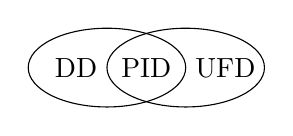
\begin{tikzpicture}
\draw (-0.5, 0) ellipse (1 and 0.5) node[left]{DD};
\draw (0.5, 0) ellipse (1 and 0.5) node[right]{UFD};
\draw (0, 0) node{PID};
\end{tikzpicture}
$$
\end{fact}

\end{frame}

\begin{frame}{The ideal class group...}

The \emph{ideal norm} is
$$ \Nm(I) = \#(\OO_K / I), \qquad I \trianglelefteq \OO_K. $$

\begin{example}
If $ K = \Q(\sqrt{-5}) $, then $ (2, 1 + \sqrt{-5}) \trianglelefteq \OO_K $ has ideal norm
\begin{align*}
\Nm((2, 1 + \sqrt{-5})) & = \#(\Z[\sqrt{-5}] / (2, 1 + \sqrt{-5})) \\
& = \#(\Z[X] / (2, 1 + X, 5 + X^2)) \\
& = \#(\F_2[X] / (1 + X, 1 + X^2))
= 2.
\end{align*}
\end{example}

\begin{fact}
\vspace{-0.3cm}
$$ \Nm(I \cdot J) = \Nm(I)\Nm(J), \qquad \Nm((x)) = \Nm(x) = \prod_{\sigma : K \to \overline{K}} \sigma(x). $$
\end{fact}

\end{frame}

\begin{frame}{The ideal class group...}

Consider the set of non-zero \emph{fractional ideals} of $ \OO_K $,
$$ \II(K) = \{x^{-1}I \subseteq K : x \in \OO_K^\times, \ I \trianglelefteq \OO_K\} \setminus \{(0)\}. $$
This is an abelian group under ideal multiplication, with identity $ (1) $ and
$$ I^{-1} = \{x \in K : xI \subseteq \OO_K\}, \qquad I \in \II(K). $$
It has a subgroup of \emph{principal fractional ideals}
$$ \PP(K) = \{(x) \in \II(K) : x \in K^\times\} \le \II(K). $$
The quotient is the \emph{ideal class group} $ \Cl(K) $.

\begin{theorem}
$ \Cl(K) $ is finite.
\end{theorem}

\begin{proof}
\emph{Geometry of numbers} gives \emph{Minkowski's bound} $ M_K \in \R_{> 0} $. Every $ [I] \in \Cl(K) $ has a representative $ I \trianglelefteq \OO_K $ with $ \Nm(I) \le M_K $.
\end{proof}

\end{frame}

\begin{frame}{The ideal class group...}

\begin{examples}
\begin{itemize}
\item If $ K = \Q, \Q(i), \Q(\sqrt{-3}) $, then $ \Cl(K) = 1 $, since $ \OO_K $ is a PID.
\item If $ K = \Q(\sqrt{-5}) $, then $ \Cl(K) \ne 1 $, since $ (2, 1 + \sqrt{-5}) \in \II(K) $ is not principal. However $ (2, 1 + \sqrt{-5})^2 = (2) $, so $ \Z / 2\Z \le \Cl(K) $. In fact $ \Cl(K) \cong \Z / 2\Z $, for instance $ (3, 1 - \sqrt{-5}) = (\tfrac{1 - \sqrt{-5}}{2}) \cdot (2, 1 + \sqrt{-5}) $.
\end{itemize}
\end{examples}

Consider $ y^2 = x^3 - 5 $. Check: $ x $ odd. In $ \Z[\sqrt{-5}] $,
\begin{align*}
(y + \sqrt{-5})(y - \sqrt{-5}) = (x)^3
& \overset{\Nm}{\implies} (y \pm \sqrt{-5}) \ \text{coprime ideals} \\
& \overset{\text{DD}}{\implies} (y \pm \sqrt{-5}) \ \text{ideal cubes}.
\end{align*}
Since $ 3 \nmid \#\Cl(\Q(\sqrt{-5})) $,
\begin{align*}
(y \pm \sqrt{-5}) = (a \pm b\sqrt{-5})^3
& \implies y \pm \sqrt{-5} = (a \pm b\sqrt{-5})^3 \\
& \implies \dots \\
& \implies \text{contradiction}
\end{align*}

\end{frame}

\begin{frame}[c]{What's next?}

\begin{itemize}
\item Quadratic forms and form class group
$$ \Cl(\Q(\sqrt{n})) \cong \Cl(\Delta_{\Q(\sqrt{n})}) $$
\item Picard group and algebraic K-theory
$$ \Cl(K) \cong \Pic(\Spec(\OO_K)) \qquad K_0(\OO_K) \cong \Z \oplus \Cl(K) $$
\item Idele class group and class field theory
$$ C^1(K) \twoheadrightarrow \Cl(K) \qquad \Cl(K) \cong \Gal(H(K) / K) $$
\item Elliptic curves and Tate--Shafarevich group
$$ \Cl(K) \cong \Sha(K) $$
\item Class number one problem and Cohen--Lenstra heuristics
$$ \Prob(\Cl(\Q(\sqrt{p})) = 1 \mid p > 0 \ \text{prime}) \approx \tfrac{3}{4} $$
\end{itemize}

\end{frame}

\end{document}